\subsection{Traffic Demand Per Subscriber}\label{subsec:behavior}

To characterize the diurnal traffic demand observed at the ISP, we first 
calculate the total traffic demand, and then the demand per subscriber
(table \ref{tab:eval-criteria}).

\begin{figure}[t]
\begin{minipage}{1\linewidth}
\centering
%
\begin{subfigure}[b]{0.49\linewidth}
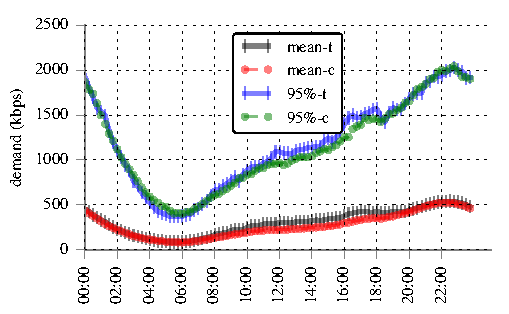
\includegraphics[width=\linewidth]{figures/weekday_demand_mean_perc95.pdf}
               \caption{Weekday traffic demand\label{fig:weekday-daily-usage}}
\end{subfigure}
%
\begin{subfigure}[b]{0.49\linewidth}
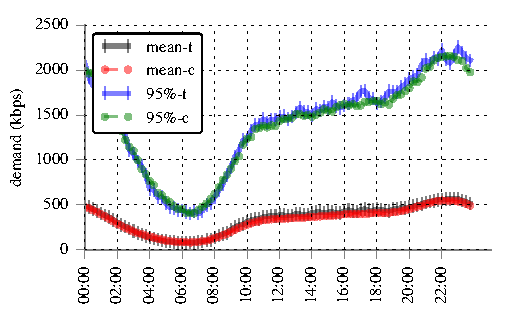
\includegraphics[width=\linewidth]{figures/weekend_demand_mean_perc95}
               \caption{Weekend traffic demand\label{fig:weekend-daily-usage}}
\end{subfigure}
%
\end{minipage}
\caption{Mean and 95th percentile traffic demand on weekdays and weekends}
\label{fig:traffic-demand-timeseries}
\end{figure}

Figure \ref{fig:traffic-demand-timeseries} shows the mean and 95th percentile
traffic demand on weekends and weekdays for the \treatment{} and \control{}
groups. We observe that the mean and 95th percentile traffic demand differs
significantly on weekdays and weekends. On weekdays, traffic demand 
increases monotonically from morning until prime-time in the evening. On 
weekends, there is a sharp rise in demand in the early morning, which 
plateaus until the next sharp rise during the evening prime-time hours.
We do not observe a trough in the demand in mid-afternoon 
(between 2:00 PM -- 6:00 PM), as is usually the case for overall usage observed 
at US Fixed access link providers \cite{sandvine20141h}.

We observed that the mean traffic demand during 7:00 PM -- 7:00 AM is 
\todo{XXX} for both \treatment{} and \control{}. However, during off peak 
daytime (work) hours, between 7:00 AM -- 7:00 PM, the \treatment{} group has a 
mean of \todo{XXX}, 20\% higher than the \control{} set.

\begin{figure*}[t]
\begin{minipage}{1\linewidth}
\centering
%
\begin{subfigure}[b]{0.33\linewidth}
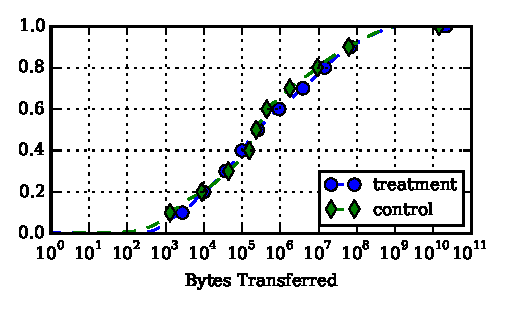
\includegraphics[width=\linewidth]{figures/cdf-all-bytes.pdf}
               \caption{Overall traffic demand\label{fig:CDF-data-rate}}
\end{subfigure}
%
\begin{subfigure}[b]{0.33\linewidth}
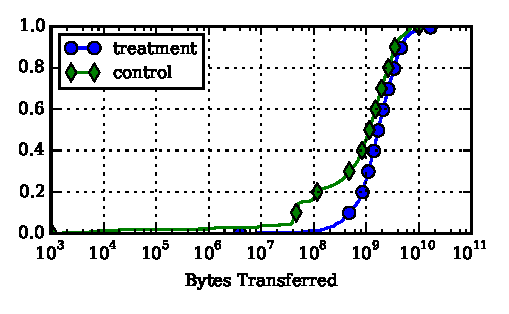
\includegraphics[width=\linewidth]{figures/cdf-per-device-max.pdf}
               \caption{Maximum traffic demand 
per subscriber\label{fig:CDF-data-rate-max}}
\end{subfigure}
%
\begin{subfigure}[b]{0.33\linewidth}
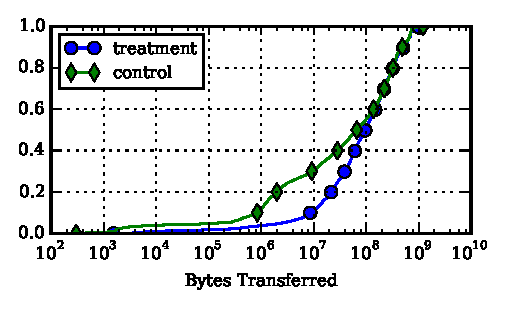
\includegraphics[width=\linewidth]{figures/cdf-per-device-perc95.pdf}
               \caption{Peak (95\%)
traffic demand per subscriber.\label{fig:CDF-data-rate-perc95}}
\end{subfigure}
%
\end{minipage}
\caption{\label{fig:traffic-demand-cdf}}
\end{figure*}


Figure \ref{fig:traffic-demand-cdf} shows the distribution of the
bytes transferred in the \treatment{} and \control{} set. Figure 
\ref{fig:CDF-data-rate}
plots all traffic seen throughout the datasets for all subscribers. The
distribution is very similar.

Figure \ref{fig:CDF-data-rate-max} plots the distribution of the
maximum demand of the subscriber. We observe that the maximum demand increases 
due 
to the service upgrade throughout the \control{} group. However, the increase is 
higher for
subscribers who have a low traffic demand. Figure \ref{fig:CDF-data-rate-perc95} 
confirms this
observation for the 95 percentile demand per subscriber.

We see that 30\% of the households from the \test set have a low 
peak demand (under 0.1 Mbps), while 40\% of the \control set households 
are under 0.1 Mbps. Thus, the absolute peak demand does not increase when 
compared to the access link capacity, but there is certainly an increase in 
peak demand of devices that had a low requirement, due to the change in 
capacity.

On investigating further, we observed that subscribers with low demand traffic 
increased their demand daily. There is negligible change in the daily peak 
demand for users
who have high demands, and a large increase for users with a low demand.
Furthermore, we observe this affect is also present in the uplink.
There could be many reasons for this increase in 
demand, such as short term activities (short videos or web browsing) 
that have a slightly higher traffic demand. Studying the applications 
responsible for such behavioral changes in traffic demand is out of the
scope of this paper and we leave it to future work.